\documentclass{beamer}

% german content
\usepackage[ngerman]{babel}

% bibliography
\usepackage[
  backend=biber,
  style=authoryear,
  citestyle=authoryear,
  autocite=footnote
]{biblatex}
\addbibresource{bibliography.bib}

% images
\usepackage{graphicx}
\graphicspath{ {./images/} }

\title{Verteilte Volltextsuche}
\subtitle{}
\author{Jonathan Neidel - 573619, Emma Calewaert - 571460} % Todo: alle rein
\date{Juni 2021}
\institute{HTW Berlin, Angewandte Informatik, Projektstudium bei Herr Hoppe}
\logo{
\includegraphics[width=1cm]{logo}}

% theme + color theme
\usetheme{Szeged}
\usecolortheme{whale}
% see: https://deic-web.uab.cat/~iblanes/beamer_gallery/index.html
\setbeamerfont{caption}{size=\Tiny}

\begin{document}
\frame{\titlepage}

\section{Projektidee}
\begin{frame}
  \begin{center}
    {\Huge Projektidee}
  \end{center}
\end{frame}

\begin{frame}
  \frametitle{Bundestagsreden}
  \begin{itemize}
    \item Protokolle als Open Data verfügbar
    \item Großer Umfang an Daten
    \item XML-Dateien*
  \end{itemize}
\end{frame}

\begin{frame}  
    \hspace*{-10.75mm}
    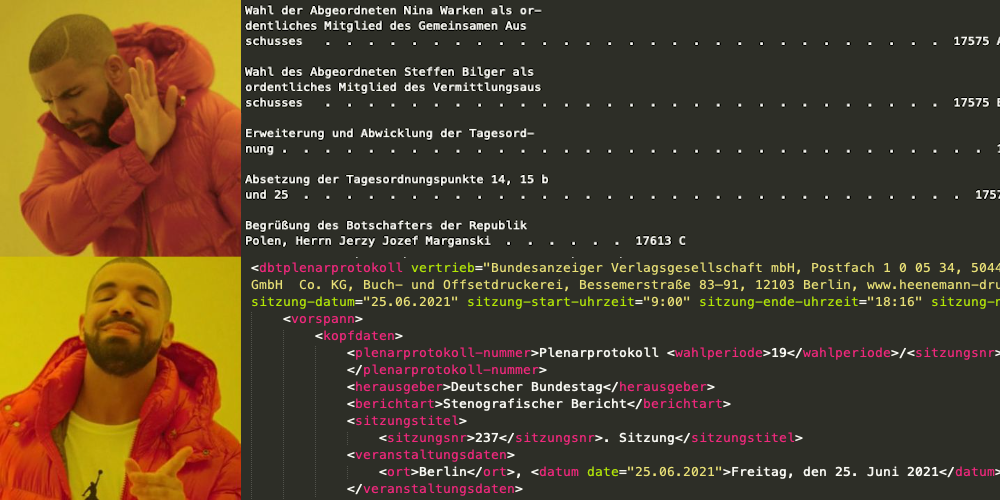
\includegraphics[width=\paperwidth]{drakememe}
\end{frame}

\begin{frame}[allowframebreaks]
  \frametitle{Basiskonzepte}
  Peer 2 Peer
  \begin{itemize}
    \item Rechnernetz
    \item Gleichtberechtigte Knoten
  \end{itemize}

  \break
  Volltextsuche
    \begin{itemize}
    \item Finden von Wörtern
    \item Handelt sich um Texte
    \item Zwei Phasen: Indexierung- und Anfragephase
  \end{itemize}
\end{frame}

\section{Komponente}
\begin{frame}
  \begin{center}
    {\Huge Komponente}
  \end{center}
\end{frame}

\begin{frame}
  \begin{center}
    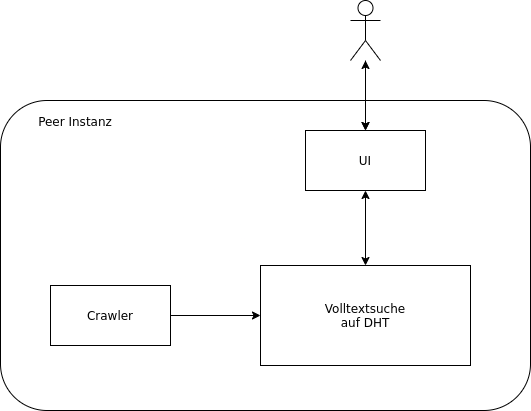
\includegraphics[width=8cm]{Komponente-einzeln}
  \end{center}
\end{frame}

\begin{frame}
  \begin{center}
    {\Huge UI}
  \end{center}
\end{frame}

\begin{frame}
  \frametitle{Crawler}

  \begin{itemize}
    \item Datenbeschaffung
    \item Vereinheitlichung
    \item Übergabe an die Volltextsuche
  \end{itemize}
\end{frame}

\begin{frame}
  \frametitle{Volltextsuche}

  Zwei Modi:
  \begin{enumerate}
    \item Einfügen von Daten
    \item Abrufen von Daten
  \end{enumerate}
\end{frame}

\begin{frame}[allowframebreaks]
  \frametitle{Einfügen von Daten}

  Füllwörter entfernen:

  \begin{itemize}
    \item Pronomen (ich, ihre, ..)
    \item Konjunktionen (und, aber, ..)
    \item Präposition (auf, bis, ..)
    \item Artikel (der, die, ..)
  \end{itemize}

  \break

  Stemming

  \bigskip

  Zurückführung auf den Wortstamm

  \medskip

  Häuser, Hauses $\rightarrow$ Haus
\end{frame}

\begin{frame}
  \frametitle{Invertierter Index}

  <++>
\end{frame}

\begin{frame}[allowframebreaks]
  \frametitle{DHT}
  P2P Aspekt des Projektes

  \begin{center}
    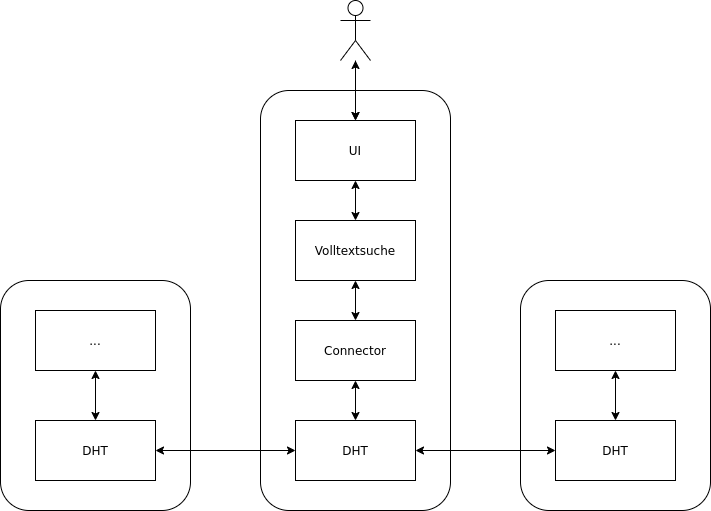
\includegraphics[width=8cm]{Komponente-verbunden}
  \end{center}
\end{frame}

\begin{frame}
  \frametitle{DHT Funktionsweise}

  <++>
\end{frame}

\section{Demo}
\begin{frame}
  \begin{center}
    {\Huge Demo}
  \end{center}
\end{frame}
% <++>

\end{document}
